
\section{Investigate at least three diverse strategies to improve your starting point}
\label{sec:Investigate diverse strategies}




\subsection{For each of these strategies: Describe the main ideas you had and hypotheses you tried, as well as their outcome after experimentally verifying or falsifying the hypotheses (via validation on (parts of) the development set). Do not hesitate to report negative outcomes.}
\label{sec:Investigate:a}

\textbf{Strategy 1: Using variable thresholds for the different classes}
\newline
Using a simple globally constant threshold for each class does work (as has been shown in \hyperref[sec:Build a simple SED system]{2.)} ), but most likely is not optimal. Factors like the heavy class imbalances or the models sensitivity to the different classes are completely ignored this way. Additionally, the different costs associated with each class also are not accounted for.
\newline
For this reason, we wanted to tune the thresholds for each of the 10 classes as well. For each class, our threshold search space consists of values from 0 to 1, in intervals of 0.05. After each validation epoch, we tune the thresholds for each class by picking the one which maximises the following utility function: $U = TP - cost_{FP}FP - cost_{FN}FN$.

\textbf{Strategy 2: Post-processing model outputs before aggregation}
\newline
Considering our aggregation strategy discussed in \hyperref[sec:Build:a]{2.) a.)}, spurious positive class predictions lasting only a few frames could potentially have a big effect on overall performance. This might even be amplified by our custom loss function and the fact that FNs are punished more heavily than FPs, i.e. our model is more pushed toward predicting positive labels when it is unsure.
\newline
Therefore, we applied a post-processing strategy to the thresholded model outputs, where positive predictions lasting only for a few frames get discarded (turned into negative ones). We tried out several values for the minimal accepted duration. Rejecting all positive predictions lasting fewer than 3 frames worked the best for us on our validation data.


\textbf{Strategy 3: Training Hyperparameter Tuning}
\newline
Our last improvement strategy consisted of trying out different values for the hyperparameters controlling the training procedure. Specifically, we looked at possible optimizers (Adam, AdamW), different batch sizes (32, 64, 128, 256) as well as different learning rates (1e-3, 1e-4, 1e-5).
\newline
In the end, using AdamW as the optimizer, a batch size of 64 and a learning rate of 1e-4 proved to be the most performant combination.

The results from applying these strategies (on their own) on top of the model described in \hyperref[sec:Build:a]{2.)} can be viewed in \hyperref[tab:comparison]{Table \ref{tab:comparison}}.

\begin{table}[h]
\centering
\begin{tabular}{|c|c|c|}
\hline
\textbf{Strategy} & \textbf{Best Validation Cost} \\
\hline
baseline (no strategy) & 40.1256 \\
\hline
Variable Thresholds & 38.275 \\
\hline
Post-processing & 40.5103 \\
\hline
Tuned Parameters & 39.8219 \\
\hline
\end{tabular}
\captionsetup{justification=centering}
\caption{Best Total average costs on validation data depending on used strategies}
\label{tab:comparison}
\end{table}
As can be seen, the most impactful strategy seems to be the one of using Variable Thresholds. Using AdamW instead of Adam also resulted in a (probably insignificant) performance increase. Post-processing the model outputs did actually decrease performance despite our expectations, so our model does not seem to produce too many false spurious positive predictions.

We also tried applying different combinations of these strategies. Interestingly, none but one of them superseded using only Variable Thresholds.  The best one we found was using Variable Thresholds in combination with Tuned Parameters, which yielded a total average cost on the validation data of 38.1383 (Figure~\ref{fig:Total Validation Cost Comparison}). No significant improvement, but at least not worse.

\begin{figure}[htbp]
    \centering
    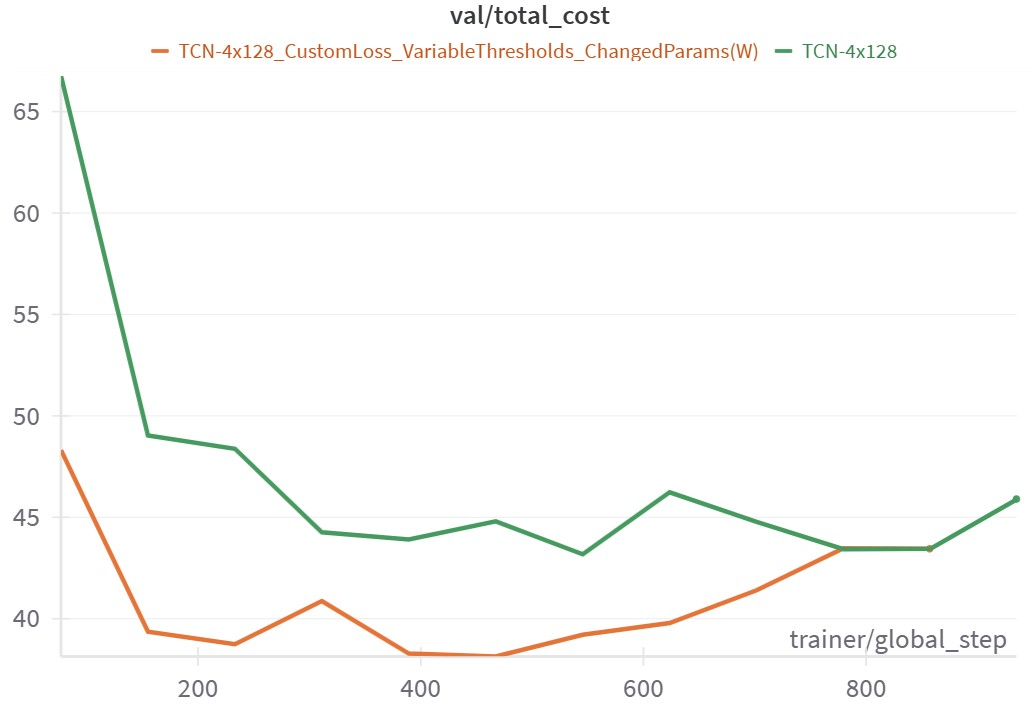
\includegraphics[width=0.8\textwidth]{figs/Total Validation Cost Comparison.jpg}
    \caption{Total validation cost comparison between base TCN and TCN with applied improvement strategies on the validation set.}
    \label{fig:Total Validation Cost Comparison}
\end{figure}

So we decided on the mentioned combination for our final model. This model now yields an unbiased cost estimate on the test dataset of 41.038 \footnote{Additional improvement strategies were explored, as can be seen in the following link: \url{https://wandb.ai/mlpc2025/mlpc2025_challenge?nw=nwusertylernavarro}.}

We then retrained our final model on the entirety of the provided data for 6 epochs (as the optimum for the best model on the validation data was achieved after 6 epochs) in order to create our predictions for the secret customer test set, utilizing the thresholds determined by the model trained on less of the data.


